\documentclass[12pt]{article}

\usepackage[utf8]{inputenc}
\usepackage{parskip}
\usepackage{setspace}
\usepackage[top=1in,bottom=1in,left=1in,right=1in]{geometry}
\usepackage{natbib}
\usepackage{hyperref}
\usepackage{rotating}
\usepackage{booktabs}
\usepackage{endnotes}
\usepackage[stable,hang]{footmisc}
\hypersetup{pdfstartpage=1,
            pdfpagemode=UseNone,
            pdfstartview=FitH,
            pdffitwindow=true,
            bookmarks=false,
            colorlinks=true,
            urlcolor=blue,
            linkcolor=blue,
            citecolor=blue}

\begin{document}

\clearpage

\thispagestyle{empty}

\begin{center}
\large Rethinking the Role of Racial Segregation in the American Foreclosure Crisis \\
\bigskip
\normalsize
Jonathan P. Latner $^{a}$\\
\end{center}

{\bf  Abstract}

Racial segregation is an important factor in understanding the foreclosure crisis, but must be understood to operate in particular and specific ways. The primary, positive impact of segregation on foreclosure risk operates prior to loan origination through the differential access to loan quality by race. Afterward, the impact of segregation is negative. Drawing on a rare dataset of loans that combine loan performance and borrower characteristics, I use a competing risks proportional hazard model to examine the impact of race and racial segregation on risk of foreclosure among borrowers.  Results indicate that Black segregation has a large, negative impact on foreclosure risk.  Instead, the strongest positive contributor to foreclosure is the negative value of the home relative to the balance of the loan (i.e. `underwater,' as measured by the put option), which is also the mechanism that explains most of the difference in the foreclosure rate by race.  The negative impact of racial segregation on foreclosure risk is the result of a mismatch between cities with high levels of segregation and cities with large declines in home prices and related foreclosures.


{\bf  Keywords:} segregation, race, foreclosure, subprime

Please cite as: Latner, Jonathan (2017).  ``Rethinking the Role of Racial Segregation in the American Foreclosure Crisis.'' \emph{City \& Community}, 16(4):447-485.

\vfill

------------------------ \\
\footnotesize
$^{a}$ Corresponding Author: Jonathan P. Latner.  E-mail:  \url{jonlatner@gmail.com}\\
The author wishes to acknowledge the following individuals for their help throughout the entire process (in alphabetical order): Jan Brülle, David Calnitsky, Matias Cocina, J. Michael Collins, Ted Gerber, Leah Gjertson, Pilar Gonalons-Pons, Gary Green, Carlotta Guistozzi, Erik Hembre, Jason Houle, Richard Latner, Timo Leper, Yifei Li, Kristina Lindemann, Heather O’Connell, Fabian Ochsenfeld, Ellen Pechman, Jacob Rugh, and Jody Schimek

\cleardoublepage

%%%%%%%%%%%%%%%%%%%%%%%%%%%%%%%%%%%%%%%%%%%%%%
%TABLES
%%%%%%%%%%%%%%%%%%%%%%%%%%%%%%%%%%%%%%%%%%%%%%
\clearpage
\section{Tables}

\begin{table}[!ht]
\caption{Descriptive statistics}
\begin{center}
\scalebox{.85}{\begin{tabular}{l*{1}{cccc}}
\hline\hline
Variables (expected sign)&        mean&          sd&         min&         max\\
\hline
& & & & \\ 
 \emph{Race \& income:} & & & \\ 
\hspace{5 mm}White (Omitted)&       0.576&       0.494&           0&           1\\
\hspace{5 mm}Black (+)&       0.138&       0.345&           0&           1\\
\hspace{5 mm}Hispanic (+)&       0.208&       0.406&           0&           1\\
\hspace{5 mm}Other (Unknown)&       0.077&       0.267&           0&           1\\
\hspace{5 mm}Income (\$10,000s) (-)&      11.392&       8.310&           2&          61\\
& & & & \\ 
 \emph{Index of segregation:} & & & \\ 
\hspace{5 mm}Black (+)&      60.537&      11.171&          22&          81\\
\hspace{5 mm}Hispanic (+)&      49.261&       9.560&          15&          70\\
\hspace{5 mm}Asian (+)&      44.741&       6.189&          20&          72\\
& & & & \\ 
 \emph{Region:} & & & \\ 
\hspace{5 mm}Northeast&       0.138&       0.345&           0&           1\\
\hspace{5 mm}Midwest&       0.145&       0.352&           0&           1\\
\hspace{5 mm}South  &       0.302&       0.459&           0&           1\\
\hspace{5 mm}West   &       0.415&       0.493&           0&           1\\
& & & & \\ 
 \emph{Put (default) option:} & & & \\ 
\hspace{5 mm}*Put (default) option (+)&      -2.109&      36.154&        -100&         296\\
\hspace{5 mm}*Put option$^2$ (+)&   1,311.533&   3,246.350&           0&      87,477\\
& & & & \\ 
 \emph{Call (prepay) option:} & & & \\ 
\hspace{5 mm}*Call (prepay) option (-)&       7.688&      41.663&        -410&          72\\
\hspace{5 mm}*Call option$^2$ (-)&   1,794.903&   3,554.471&           0&     168,100\\
& & & & \\ 
 \emph{Loan:} & & & \\ 
\hspace{5 mm}$<$ 620 (Omitted)&       0.254&       0.435&           0&           1\\
\hspace{5 mm}620-679 (-)&       0.299&       0.458&           0&           1\\
\hspace{5 mm}680-719 (-)&       0.182&       0.386&           0&           1\\
\hspace{5 mm}$>=$ 720 (-)&       0.265&       0.441&           0&           1\\
\hspace{5 mm}High Cost Loan ($>=$ 300 BPS indicator) (+)&       0.418&       0.493&           0&           1\\
\hspace{5 mm}Loan to value (LTV) (+)&      80.861&      14.751&           1&         125\\
\hspace{5 mm}Purchase (vs. refinance) indicator (+)&       0.468&       0.499&           0&           1\\
\hspace{5 mm}*ARM (vs. FRM) indicator (+)&       0.687&       0.464&           0&           1\\
\hspace{5 mm}*Modification indicator (-)&       0.145&       0.352&           0&           1\\
\hspace{5 mm}Payment to income (PTI) $>$ 31\% indicator (+)&       0.139&       0.346&           0&           1\\
& & & & \\ 
 \emph{Dependent variables:} & & & \\ 
\hspace{5 mm}Current&       0.311&       0.463&           0&           1\\
\hspace{5 mm}Prepay &       0.423&       0.494&           0&           1\\
\hspace{5 mm}Foreclosure&       0.266&       0.442&           0&           1\\
\hline\hline
\multicolumn{5}{l}{\footnotesize As of last period of observation}\\
\multicolumn{5}{l}{\footnotesize * Indicates time-varying covariate}\\
\end{tabular}
}
\label{descriptives_paper}
\end{center}
\end{table}

\begin{sidewaystable}[!ht]
\caption{Competing risks hazard model}
\begin{center}
\scalebox{.7}{{
\def\sym#1{\ifmmode^{#1}\else\(^{#1}\)\fi}
\begin{tabular}{l*{10}{c}}
\hline\hline
                    &\multicolumn{1}{c}{(1)}         &\multicolumn{1}{c}{(2)}         &\multicolumn{1}{c}{(3)}         &\multicolumn{1}{c}{(4)}         &\multicolumn{1}{c}{(5)}         &\multicolumn{1}{c}{(6)}         &\multicolumn{1}{c}{(7)}         &\multicolumn{1}{c}{(8)}         &\multicolumn{1}{c}{(9)}         &\multicolumn{1}{c}{(10)}         \\
                    &Race \& inc.         & Segregation         &Race, inc., \& seg         &+ Interaction         &+ Loan controls         &+ Options (Main)         &   Northeast         &     Midwest         &       South         &        West         \\
                    &        b/se         &        b/se         &        b/se         &        b/se         &        b/se         &        b/se         &        b/se         &        b/se         &        b/se         &        b/se         \\
\hline
& & & & & \\ 
 \emph{Borrower:} & & & & & \\ 
Black               &       1.519\sym{***}&                     &       1.599\sym{***}&       1.567\sym{***}&       1.217\sym{***}&       1.038\sym{*}  &       1.235\sym{***}&       1.233\sym{***}&       1.030         &       0.956\sym{*}  \\
                    &     (0.023)         &                     &     (0.024)         &     (0.024)         &     (0.019)         &     (0.017)         &     (0.040)         &     (0.026)         &     (0.016)         &     (0.019)         \\
Hispanic            &       1.979\sym{***}&                     &       2.063\sym{***}&       2.041\sym{***}&       1.652\sym{***}&       1.258\sym{***}&       1.380\sym{***}&       1.325\sym{***}&       1.319\sym{***}&       1.262\sym{***}\\
                    &     (0.021)         &                     &     (0.022)         &     (0.023)         &     (0.019)         &     (0.015)         &     (0.041)         &     (0.033)         &     (0.019)         &     (0.013)         \\
Other               &       1.310\sym{***}&                     &       1.349\sym{***}&       1.334\sym{***}&       1.301\sym{***}&       1.221\sym{***}&       1.217\sym{***}&       1.294\sym{***}&       1.325\sym{***}&       1.147\sym{***}\\
                    &     (0.023)         &                     &     (0.023)         &     (0.024)         &     (0.024)         &     (0.022)         &     (0.064)         &     (0.049)         &     (0.036)         &     (0.015)         \\
Income (\$10,000s)  &       0.978\sym{***}&                     &       0.981\sym{***}&       0.981\sym{***}&       0.999         &       1.001         &       0.989\sym{***}&       0.995\sym{**} &       1.000         &       1.004\sym{***}\\
                    &     (0.001)         &                     &     (0.001)         &     (0.001)         &     (0.001)         &     (0.001)         &     (0.002)         &     (0.002)         &     (0.001)         &     (0.001)         \\
& & & & & \\ 
 \emph{Segregation:} & & & & & \\ 
Black               &                     &       0.985\sym{***}&       0.985\sym{***}&       0.985\sym{***}&       0.988\sym{***}&       0.988\sym{***}&       0.977\sym{***}&       0.986\sym{***}&       0.998         &       1.000         \\
                    &                     &     (0.001)         &     (0.001)         &     (0.001)         &     (0.001)         &     (0.001)         &     (0.002)         &     (0.001)         &     (0.001)         &     (0.001)         \\
Hispanic            &                     &       1.008\sym{***}&       1.003\sym{***}&       1.003\sym{***}&       1.008\sym{***}&       1.003\sym{***}&       1.016\sym{***}&       1.005\sym{***}&       0.988\sym{***}&       1.000         \\
                    &                     &     (0.001)         &     (0.001)         &     (0.001)         &     (0.001)         &     (0.001)         &     (0.002)         &     (0.001)         &     (0.001)         &     (0.001)         \\
Asian               &                     &       0.997\sym{***}&       0.999         &       0.999         &       1.000         &       1.012\sym{***}&       1.000         &       0.995\sym{*}  &       1.022\sym{***}&       1.002\sym{*}  \\
                    &                     &     (0.001)         &     (0.001)         &     (0.001)         &     (0.001)         &     (0.001)         &     (0.003)         &     (0.002)         &     (0.001)         &     (0.001)         \\
& & & & & \\ 
 \emph{Race \& segregation interaction:} & & & & & \\ 
Black \& Black segregation&                     &                     &                     &       1.007\sym{***}&       1.007\sym{***}&       1.005\sym{***}&       1.004         &       1.002         &       0.997         &       0.998         \\
                    &                     &                     &                     &     (0.001)         &     (0.001)         &     (0.001)         &     (0.004)         &     (0.002)         &     (0.002)         &     (0.002)         \\
Hispanic \& Black segregation&                     &                     &                     &       0.996\sym{***}&       0.995\sym{***}&       1.002\sym{*}  &       0.998         &       0.996         &       1.001         &       1.001         \\
                    &                     &                     &                     &     (0.001)         &     (0.001)         &     (0.001)         &     (0.003)         &     (0.002)         &     (0.002)         &     (0.001)         \\
Other \& Black segregation&                     &                     &                     &       0.997\sym{*}  &       0.995\sym{**} &       1.003\sym{*}  &       1.012         &       0.985\sym{***}&       1.008\sym{*}  &       1.002         \\
                    &                     &                     &                     &     (0.001)         &     (0.001)         &     (0.002)         &     (0.007)         &     (0.003)         &     (0.004)         &     (0.001)         \\
& & & & & \\ 
 \emph{Put (default) option:} & & & & & \\ 
Put option          &                     &                     &                     &                     &                     &       1.038\sym{***}&       1.055\sym{***}&       1.046\sym{***}&       1.033\sym{***}&       1.040\sym{***}\\
                    &                     &                     &                     &                     &                     &     (0.000)         &     (0.001)         &     (0.001)         &     (0.000)         &     (0.000)         \\
Put option$^2$      &                     &                     &                     &                     &                     &       1.000\sym{***}&       1.000\sym{***}&       1.000\sym{***}&       1.000\sym{***}&       1.000\sym{***}\\
                    &                     &                     &                     &                     &                     &     (0.000)         &     (0.000)         &     (0.000)         &     (0.000)         &     (0.000)         \\
& & & & & \\ 
 \emph{Call (prepay) option:} & & & & & \\ 
Call option         &                     &                     &                     &                     &                     &       1.015\sym{***}&       1.026\sym{***}&       1.019\sym{***}&       1.016\sym{***}&       1.012\sym{***}\\
                    &                     &                     &                     &                     &                     &     (0.000)         &     (0.001)         &     (0.000)         &     (0.000)         &     (0.000)         \\
Call option$^2$     &                     &                     &                     &                     &                     &       1.000\sym{***}&       1.000\sym{***}&       1.000\sym{***}&       1.000\sym{***}&       1.000\sym{***}\\
                    &                     &                     &                     &                     &                     &     (0.000)         &     (0.000)         &     (0.000)         &     (0.000)         &     (0.000)         \\
\hline
Number of Observations&   7,927,358         &   7,927,358         &   7,927,358         &   7,927,358         &   7,927,358         &   7,927,358         &   2,955,494         &   2,715,450         &   6,282,241         &   7,848,442         \\
Number of Subjects  &     192,617         &     192,617         &     192,617         &     192,617         &     192,617         &     192,617         &      65,407         &      70,788         &     144,915         &     199,378         \\
Number of Failures (Foreclosure)&      50,874         &      50,874         &      50,874         &      50,874         &      50,874         &      50,874         &       8,755         &      21,065         &      35,711         &      62,607         \\
Number of Competing (Prepay)&      81,117         &      81,117         &      81,117         &      81,117         &      81,117         &      81,117         &      30,280         &      29,402         &      60,041         &      82,005         \\
\hspace{5mm}        &                     &                     &                     &                     &                     &                     &                     &                     &                     &                     \\
\emph{Control variables:}&                     &                     &                     &                     &                     &                     &                     &                     &                     &                     \\
Year of origination &         Yes         &         Yes         &         Yes         &         Yes         &         Yes         &         Yes         &         Yes         &         Yes         &         Yes         &         Yes         \\
Region              &         Yes         &         Yes         &         Yes         &         Yes         &         Yes         &         Yes         &         N/A         &         N/A         &         N/A         &         N/A         \\
Race \& Income interaction&         Yes         &          No         &         Yes         &         Yes         &         Yes         &         Yes         &         Yes         &         Yes         &         Yes         &         Yes         \\
Loan performance (LTV, ARM, etc.)&          No         &          No         &          No         &          No         &         Yes         &         Yes         &         Yes         &         Yes         &         Yes         &         Yes         \\
\hline\hline
\multicolumn{11}{l}{\footnotesize National models are run on a 20\% sample.  Regional models are run on a 50\% regional sample.}\\
\multicolumn{11}{l}{\footnotesize \sym{*} \(p<0.05\), \sym{**} \(p<0.01\), \sym{***} \(p<0.001\)}\\
\end{tabular}
}
}
\label{stcrreg_default}
\end{center}
\end{sidewaystable}

\begin{sidewaystable}[!ht]
\caption{Competing risks hazard model - control variables from table \ref{stcrreg_default}}
\begin{center}
\scalebox{.7}{{
\def\sym#1{\ifmmode^{#1}\else\(^{#1}\)\fi}
\begin{tabular}{l*{10}{c}}
\hline\hline
                    &\multicolumn{1}{c}{(1)}         &\multicolumn{1}{c}{(2)}         &\multicolumn{1}{c}{(3)}         &\multicolumn{1}{c}{(4)}         &\multicolumn{1}{c}{(5)}         &\multicolumn{1}{c}{(6)}         &\multicolumn{1}{c}{(7)}         &\multicolumn{1}{c}{(8)}         &\multicolumn{1}{c}{(9)}         &\multicolumn{1}{c}{(10)}         \\
                    &Race \& inc.         & Segregation         &Race, inc., \& seg         &+ Interaction         &+ Loan controls         &+ Options (Main)         &   Northeast         &     Midwest         &       South         &        West         \\
                    &        b/se         &        b/se         &        b/se         &        b/se         &        b/se         &        b/se         &        b/se         &        b/se         &        b/se         &        b/se         \\
\hline
& & & & & \\ 
 \emph{Year of origination:} & & & & & \\ 
2005                &       1.761\sym{***}&       1.827\sym{***}&       1.755\sym{***}&       1.755\sym{***}&       1.505\sym{***}&       0.896\sym{***}&       0.730\sym{***}&       0.803\sym{***}&       0.952\sym{*}  &       0.951\sym{**} \\
                    &     (0.029)         &     (0.030)         &     (0.028)         &     (0.028)         &     (0.025)         &     (0.016)         &     (0.029)         &     (0.017)         &     (0.020)         &     (0.017)         \\
2006                &       2.541\sym{***}&       2.696\sym{***}&       2.523\sym{***}&       2.521\sym{***}&       2.084\sym{***}&       0.762\sym{***}&       0.552\sym{***}&       0.678\sym{***}&       0.811\sym{***}&       0.782\sym{***}\\
                    &     (0.040)         &     (0.042)         &     (0.040)         &     (0.040)         &     (0.034)         &     (0.014)         &     (0.023)         &     (0.015)         &     (0.018)         &     (0.014)         \\
2007                &       2.268\sym{***}&       2.324\sym{***}&       2.263\sym{***}&       2.262\sym{***}&       2.060\sym{***}&       0.621\sym{***}&       0.391\sym{***}&       0.573\sym{***}&       0.671\sym{***}&       0.640\sym{***}\\
                    &     (0.043)         &     (0.044)         &     (0.043)         &     (0.043)         &     (0.041)         &     (0.013)         &     (0.021)         &     (0.018)         &     (0.018)         &     (0.013)         \\
& & & & & \\ 
 \emph{Race \& income interaction:} & & & & & \\ 
Black \& income     &       1.023\sym{***}&                     &       1.023\sym{***}&       1.023\sym{***}&       1.008\sym{***}&       1.005\sym{*}  &       1.029\sym{***}&       0.999         &       1.010\sym{***}&       1.012\sym{***}\\
                    &     (0.002)         &                     &     (0.002)         &     (0.002)         &     (0.002)         &     (0.002)         &     (0.005)         &     (0.004)         &     (0.002)         &     (0.003)         \\
Hispanic \& income  &       1.037\sym{***}&                     &       1.037\sym{***}&       1.037\sym{***}&       1.022\sym{***}&       1.016\sym{***}&       1.025\sym{***}&       1.026\sym{***}&       1.018\sym{***}&       1.012\sym{***}\\
                    &     (0.001)         &                     &     (0.001)         &     (0.001)         &     (0.001)         &     (0.002)         &     (0.005)         &     (0.005)         &     (0.002)         &     (0.001)         \\
Other \& income     &       1.011\sym{***}&                     &       1.010\sym{***}&       1.011\sym{***}&       1.005\sym{*}  &       1.007\sym{***}&       1.015\sym{*}  &       1.007         &       1.017\sym{***}&       1.006\sym{***}\\
                    &     (0.002)         &                     &     (0.002)         &     (0.002)         &     (0.002)         &     (0.002)         &     (0.007)         &     (0.006)         &     (0.003)         &     (0.002)         \\
& & & & & \\ 
 \emph{Region:} & & & & & \\ 
 \emph{Northeast (ommitted)} & & & & & \\ 
Midwest             &       2.548\sym{***}&       2.682\sym{***}&       2.621\sym{***}&       2.611\sym{***}&       2.348\sym{***}&       1.648\sym{***}&                     &                     &                     &                     \\
                    &     (0.052)         &     (0.056)         &     (0.055)         &     (0.055)         &     (0.050)         &     (0.036)         &                     &                     &                     &                     \\
South               &       1.845\sym{***}&       1.720\sym{***}&       1.538\sym{***}&       1.569\sym{***}&       1.690\sym{***}&       1.118\sym{***}&                     &                     &                     &                     \\
                    &     (0.035)         &     (0.034)         &     (0.031)         &     (0.032)         &     (0.035)         &     (0.024)         &                     &                     &                     &                     \\
West                &       2.583\sym{***}&       2.263\sym{***}&       2.057\sym{***}&       2.073\sym{***}&       2.659\sym{***}&       1.668\sym{***}&                     &                     &                     &                     \\
                    &     (0.047)         &     (0.044)         &     (0.041)         &     (0.042)         &     (0.055)         &     (0.035)         &                     &                     &                     &                     \\
& & & & & \\ 
 \emph{Loan characteristics:} & & & & & \\ 
 \emph{FICO $<$ 620 (ommitted)} & & & & & \\ 
FICO (620-679)      &                     &                     &                     &                     &       0.951\sym{***}&       0.966\sym{**} &       1.154\sym{***}&       0.953\sym{**} &       1.010         &       0.974\sym{*}  \\
                    &                     &                     &                     &                     &     (0.011)         &     (0.012)         &     (0.032)         &     (0.016)         &     (0.014)         &     (0.013)         \\
FICO (680-719)      &                     &                     &                     &                     &       0.794\sym{***}&       0.814\sym{***}&       0.964         &       0.791\sym{***}&       0.868\sym{***}&       0.786\sym{***}\\
                    &                     &                     &                     &                     &     (0.012)         &     (0.013)         &     (0.036)         &     (0.020)         &     (0.016)         &     (0.012)         \\
FICO ($>=$ 720)     &                     &                     &                     &                     &       0.510\sym{***}&       0.563\sym{***}&       0.669\sym{***}&       0.509\sym{***}&       0.599\sym{***}&       0.575\sym{***}\\
                    &                     &                     &                     &                     &     (0.008)         &     (0.010)         &     (0.030)         &     (0.016)         &     (0.013)         &     (0.009)         \\
High cost loan (\textgreater = 300 BPS indicator)&                     &                     &                     &                     &       1.351\sym{***}&       1.296\sym{***}&       1.414\sym{***}&       1.239\sym{***}&       1.264\sym{***}&       1.357\sym{***}\\
                    &                     &                     &                     &                     &     (0.015)         &     (0.014)         &     (0.042)         &     (0.023)         &     (0.017)         &     (0.013)         \\
Loan to value (LTV) &                     &                     &                     &                     &       1.033\sym{***}&       1.005\sym{***}&       0.994\sym{***}&       0.984\sym{***}&       1.002\sym{**} &       1.009\sym{***}\\
                    &                     &                     &                     &                     &     (0.000)         &     (0.000)         &     (0.001)         &     (0.001)         &     (0.001)         &     (0.000)         \\
Purchase (vs. refinance) indicator&                     &                     &                     &                     &       1.187\sym{***}&       1.265\sym{***}&       1.105\sym{***}&       1.288\sym{***}&       1.309\sym{***}&       1.254\sym{***}\\
                    &                     &                     &                     &                     &     (0.012)         &     (0.013)         &     (0.028)         &     (0.020)         &     (0.017)         &     (0.012)         \\
ARM indicator       &                     &                     &                     &                     &       1.492\sym{***}&       1.490\sym{***}&       1.330\sym{***}&       1.225\sym{***}&       1.466\sym{***}&       1.605\sym{***}\\
                    &                     &                     &                     &                     &     (0.017)         &     (0.018)         &     (0.036)         &     (0.021)         &     (0.019)         &     (0.019)         \\
Modification indicator&                     &                     &                     &                     &       1.164\sym{***}&       0.901\sym{***}&       0.800\sym{***}&       1.135\sym{***}&       1.025         &       0.781\sym{***}\\
                    &                     &                     &                     &                     &     (0.017)         &     (0.015)         &     (0.033)         &     (0.028)         &     (0.020)         &     (0.012)         \\
PTI $>$ 31\% indicator&                     &                     &                     &                     &       1.053\sym{***}&       1.024         &       1.058\sym{*}  &       1.070\sym{**} &       1.019         &       0.996         \\
                    &                     &                     &                     &                     &     (0.014)         &     (0.014)         &     (0.029)         &     (0.022)         &     (0.017)         &     (0.013)         \\
\hline\hline
\multicolumn{11}{l}{\footnotesize National models are run on a 20\% sample.  Regional models are run on a 50\% regional sample.}\\
\multicolumn{11}{l}{\footnotesize \sym{*} \(p<0.05\), \sym{**} \(p<0.01\), \sym{***} \(p<0.001\)}\\
\end{tabular}
}
}
\label{control}
\end{center}
\end{sidewaystable}

\begin{sidewaystable}[!ht]
\caption{Marginal effect on the risk of foreclosure from the main model}
\begin{center}
\scalebox{1}{%%%%%%%%
%Effect size paper
%%%%%%%%

{
\def\sym#1{\ifmmode^{#1}\else\(^{#1}\)\fi}
\begin{tabular}{l*{8}{l}} \hline\hline
& \multicolumn{4}{l}{United States} & Northeast & Midwest & South & West \\ \cmidrule(l){2-5} \cmidrule(l){6-9}

& \multicolumn{1}{c}{mean} & \multicolumn{1}{c}{mean + 1 sd} & \multicolumn{1}{c}{\emph{exp($\beta$)}} & \multicolumn{1}{c}{\emph{$\beta$}} & \multicolumn{1}{c}{\emph{$\beta$}} & \multicolumn{1}{c}{\emph{$\beta$}} & \multicolumn{1}{c}{\emph{$\beta$}} & \multicolumn{1}{c}{\emph{$\beta$}} \\ \hline

\multicolumn{9}{l}{}\\
\multicolumn{9}{l}{\emph{Continuous variables (Marginal effect of 1 SD increase from the mean):}} \\

\hspace{5mm} Put option&2.504&38.15&3.041&1.112\sym{***}&1.478\sym{***}&1.276\sym{***}&0.978\sym{***}&1.163\sym{***}\\
\hspace{5mm} Call option&8.418&45.059&1.83&0.604\sym{***}&1.033\sym{***}&0.736\sym{***}&0.658\sym{***}&0.5\sym{***}\\
\hspace{5mm} LTV &80.783&95.484&1.073&0.071\sym{***}&-0.082\sym{***}&-0.24\sym{***}&0.024\sym{**}&0.139\sym{***}\\
\hspace{5mm} Income (\$10,000s)&11.656&20.148&1.05&0.049\sym{***}&-0.01&0.002&0.053\sym{***}&0.07\sym{***}\\
\hspace{5mm} Asian segregation&44.847&51.059&1.075&0.072\sym{***}&0.002&-0.03\sym{*}&0.137\sym{***}&0.014\sym{*}\\
\hspace{5mm} Hispanic segregation&49.569&59.137&1.025&0.024\sym{**}&0.154\sym{***}&0.05\sym{***}&-0.112\sym{***}&-0.004\\
\hspace{5mm} Black segregation&60.85&71.954&0.886&-0.121\sym{***}&-0.241\sym{***}&-0.174\sym{***}&-0.015&0.001\\

\multicolumn{9}{l}{}\\
\multicolumn{9}{l}{\emph{Categorical variables:}} \\

\hspace{5mm} ARM indicator&&&1.49&0.399\sym{***}&0.285\sym{***}&0.203\sym{***}&0.383\sym{***}&0.473\sym{***}\\
\hspace{5mm} Hispanic to white&&&1.257&0.229\sym{***}&0.323\sym{***}&0.281\sym{***}&0.277\sym{***}&0.233\sym{***}\\
\hspace{5mm} High cost loan indicator&&&1.296&0.259\sym{***}&0.347\sym{***}&0.215\sym{***}&0.234\sym{***}&0.306\sym{***}\\
\hspace{5mm} Purchase to refinance&&&1.265&0.235\sym{***}&0.1\sym{***}&0.253\sym{***}&0.269\sym{***}&0.226\sym{***}\\
\hspace{5mm} Black to white&&&1.038&0.037\sym{*}&0.211\sym{***}&0.21\sym{***}&0.029&-0.045\sym{*}\\
\hspace{5mm} PTI $>$ 31\% indicator&&&1.024&0.023&0.057\sym{*}&0.068\sym{**}&0.019&-0.004\\
\hspace{5mm} Modification indicator&&&0.901&-0.104\sym{***}&-0.223\sym{***}&0.126\sym{***}&0.025&-0.248\sym{***}\\
\hspace{5mm} FICO $>=$ 720 to FICO $<$ 620&&&0.563&-0.575\sym{***}&-0.401\sym{***}&-0.675\sym{***}&-0.513\sym{***}&-0.553\sym{***}\\

\hline\hline
\multicolumn{9}{l}{\footnotesize \sym{*} \(p<0.05\), \sym{**} \(p<0.01\), \sym{***} \(p<0.001\)}\\
\end{tabular}
}
}
\label{effect_size}
\end{center}
\end{sidewaystable}

%%%%%%%%%%%%%%%%%%%%%%%%%%%%%%%%%%%%%%%%%%%%%%
%FIGURES
%%%%%%%%%%%%%%%%%%%%%%%%%%%%%%%%%%%%%%%%%%%%%%
\clearpage
\section{Figures}

\begin{figure}[htp!]
\centering
\caption{Correlation between segregation and housing price index (HPI)}
\centering
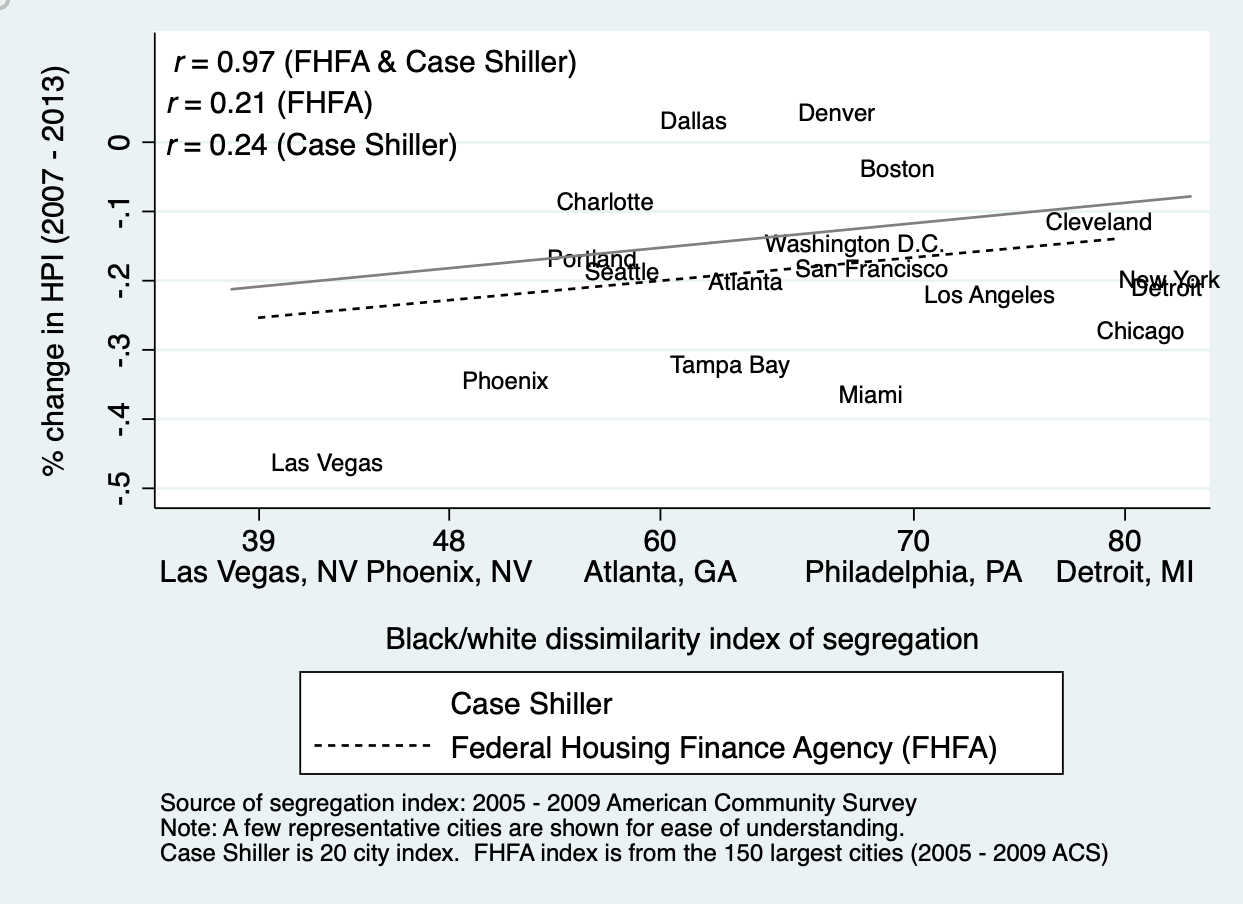
\includegraphics[scale=.75]{../graphs/segregation_hpi}
\label{segregation_hpi}
\end{figure}

\begin{figure}[htp!]
\centering
\caption{Correlation between RealtyTrac and CTS foreclosures across metropolitan
areas}
\centering
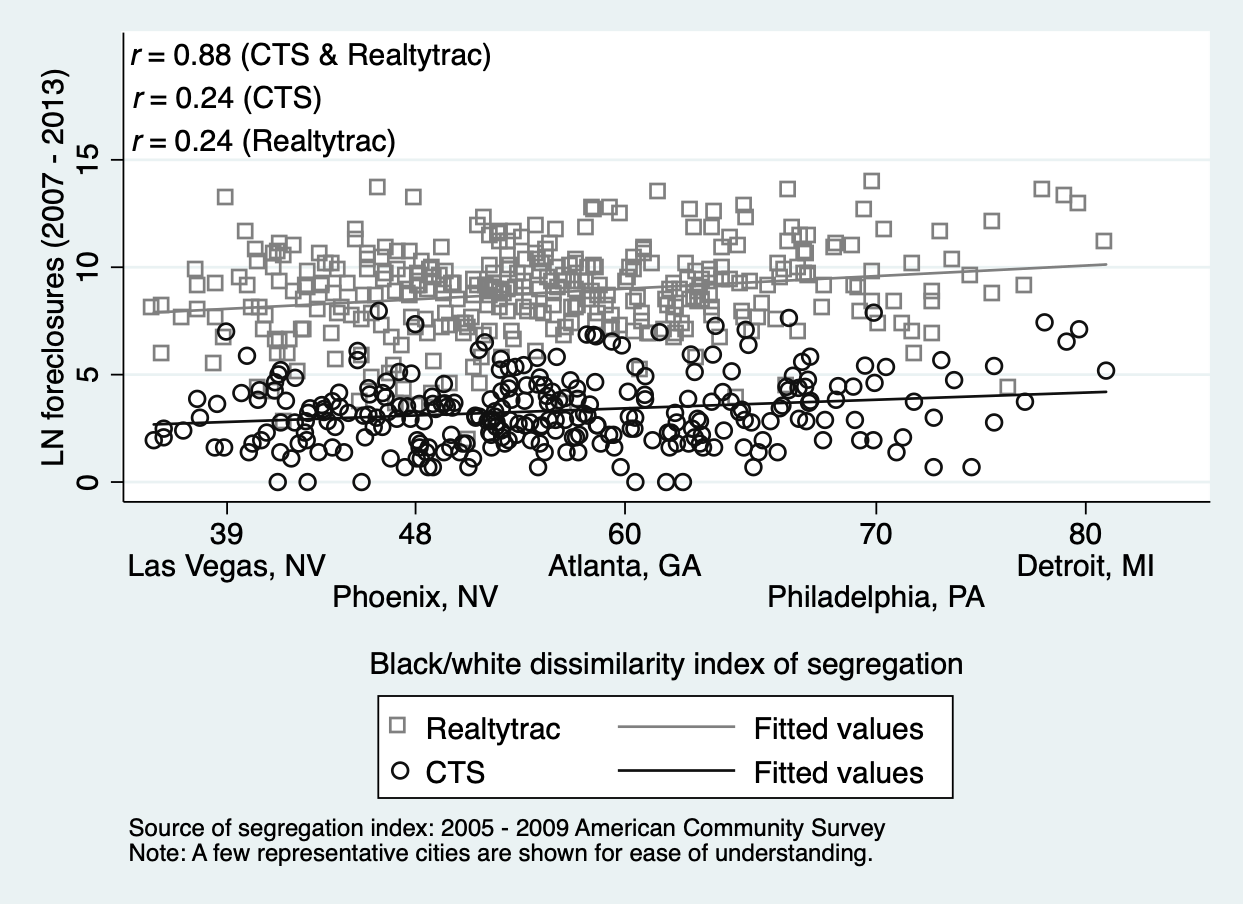
\includegraphics[scale=.75]{../graphs/cor_cts_realtytrac}
\label{cor_cts_realtytrac}
\end{figure}


\clearpage
\begin{figure}[htp!]
\centering
\caption{Model adjusted cumulative foreclosure rate by race}
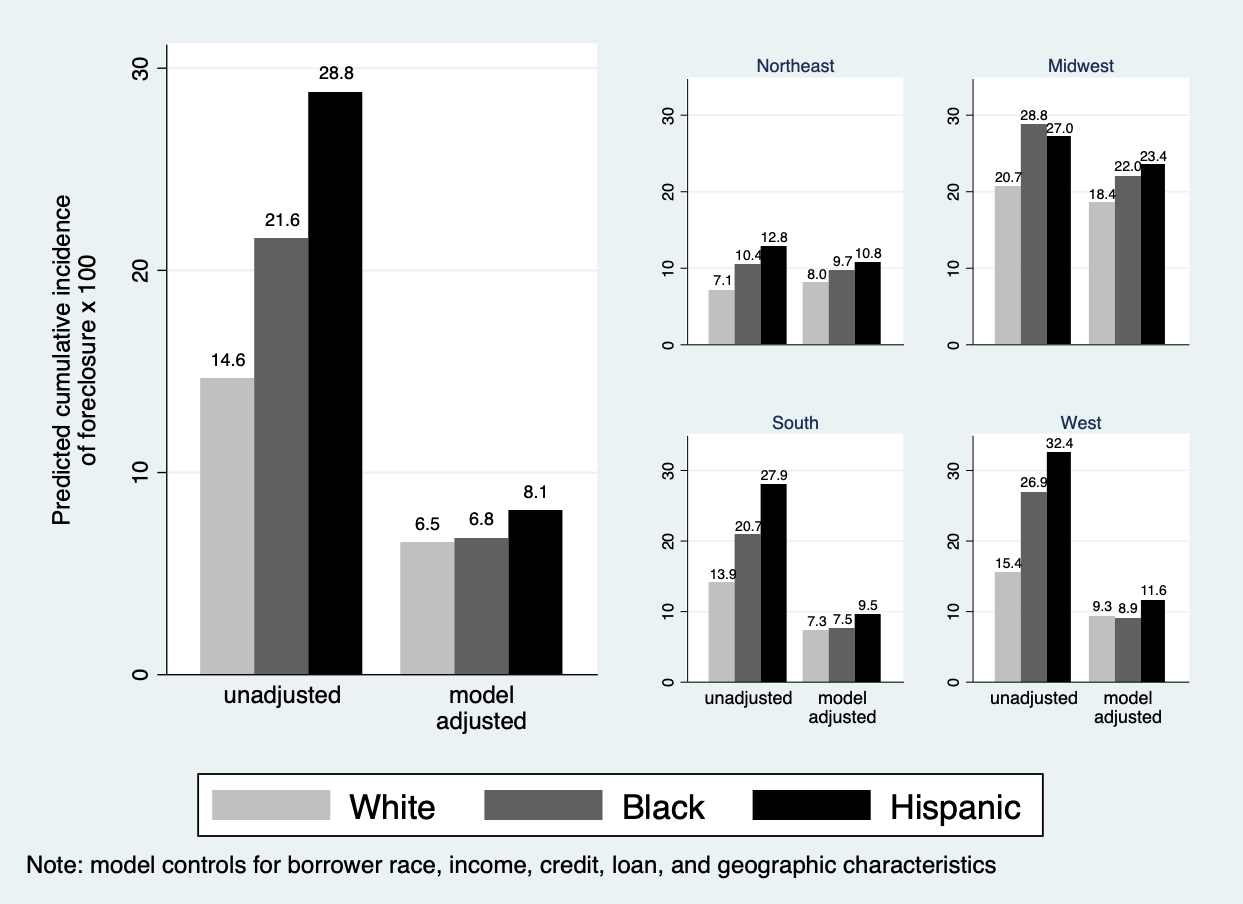
\includegraphics[scale=.75]{../graphs/predict_basecif_center_race_region}
\label{predict_basecif_race_policy}
\end{figure}

\begin{figure}[htp!]
\centering
\caption{Interaction between race and black segregation}
\centering
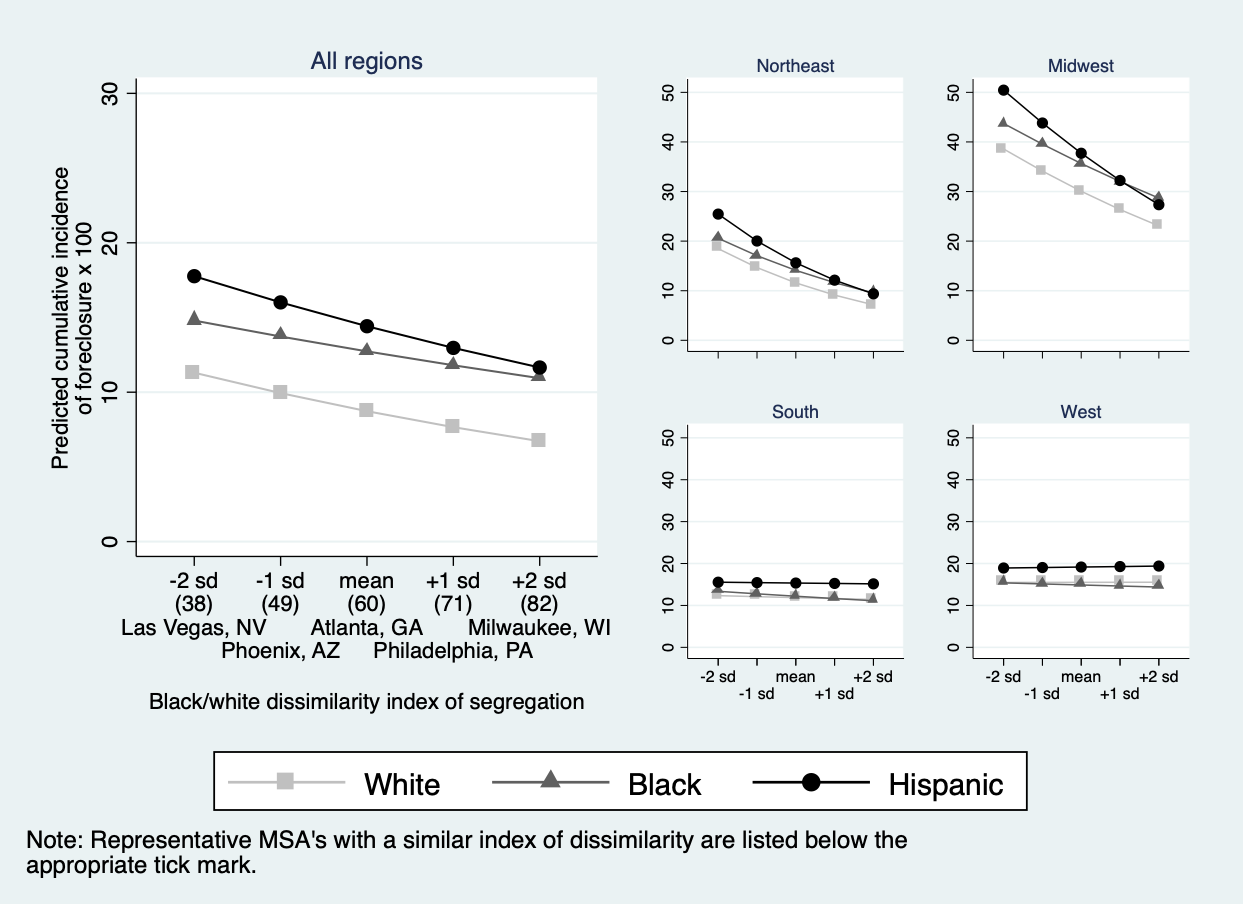
\includegraphics[scale=.75]{../graphs/predict_basecif_segregation_center_race_region}
\label{predict_basecif_segregation}
\end{figure}

\end{document}


